% !TEX root = ../main.tex
% chktex-file 21
% chktex-file 46
\section{Graph Coarsening}%
\label{sec:coarse}

We will now see how the size of a graph $G$ can be reduced via \textit{graph coarsening}.
The resulting coarsened graph $G_c$ should ideally be structurally similar to $G$, i.e.\  it should have a similar spectrum.
In this section we will first define the class of coarsening operators $C$ and give an intuition on how they change the shape of a graph.
Then we will describe a randomized algorithm to compute such a coarsening.

\subsection{Definition of the Coarsening Operator}%
\label{sec:coarse:formal}

The core idea of graph coarsening is to replace clusters of vertices in the original graph $G$ by single vertices in the coarsened graph $G_c$.
Formally this means that the original vertices $\mathcal{V} = \{ v_1, \dots, v_N \}$ are mapped to a smaller vertex set $\mathcal{V}_c = \{ v'_1, \dots, v'_n \}$ via a surjective mapping $\varphi: \mathcal{V} \to \mathcal{V}_c$.
The original edges $(v_i, v_j) \in \mathcal{E}$ are mapped to $(\varphi(v_i), \varphi(v_j))$, resulting in a reduced edge set $\mathcal{E}_c$ that contains every edge for which $\varphi(v_i) \neq \varphi(v_j)$.
\Cref{fig:coarse:example:original,fig:coarse:example:coarsened} show an exemplary graph coarsening.
To reverse the coarsening mapping, we define $\varphi^{-1}: \mathcal{V}_c \to \mathcal{P}(\mathcal{V})$ as the mapping from a coarsened vertex to the set of original vertices it represents.
\begin{figure}[ht]
	\centering
	\begin{subfigure}{0.33\textwidth}
		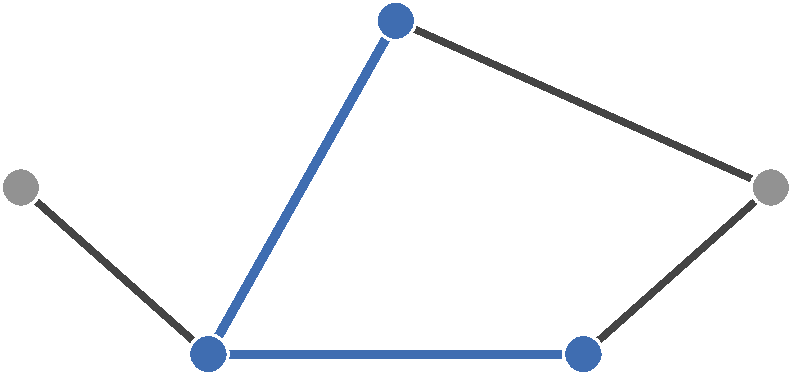
\includegraphics[width=0.9\linewidth]{gfx/coarse/example/original.pdf}
		\caption{Original $G$}\label{fig:coarse:example:original}
	\end{subfigure}%
	\begin{subfigure}{0.33\textwidth}
		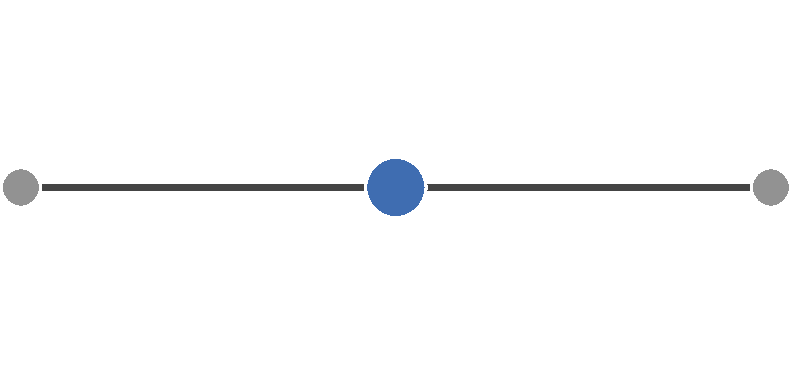
\includegraphics[width=0.9\linewidth]{gfx/coarse/example/coarsened.pdf}
		\caption{Coarsened $G_c$}\label{fig:coarse:example:coarsened}
	\end{subfigure}%
	\begin{subfigure}{0.33\textwidth}
		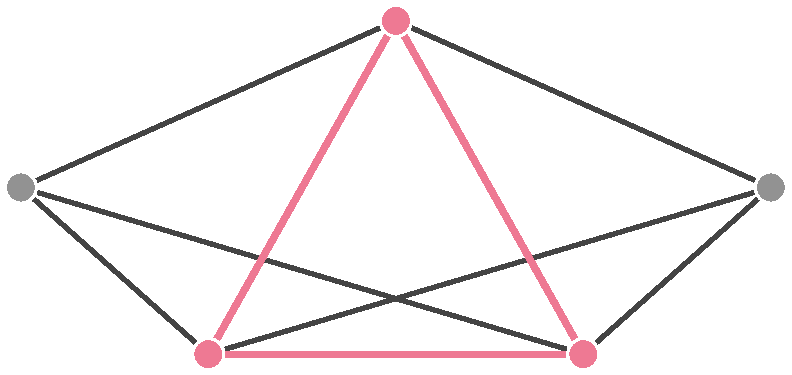
\includegraphics[width=0.9\linewidth]{gfx/coarse/example/reexpanded.pdf}
		\caption{Approximated $\widetilde{G}$}\label{fig:coarse:example:reexpanded}
	\end{subfigure}
	\caption{%
		Example showing the effect of coarsening $G$ when merging the blue vertices into a single vertex.
		The graph $\widetilde{G}$ on the right shows the result of re-expanding $G_c$.
	}\label{fig:coarse:example}
\end{figure}

In the last section we saw how graphs can be described via their Laplacian $L$.
Since our goal is to analyze the effects of coarsening on the overall characteristics of a graph, we will now describe a coarsening $\varphi$ as an operation that acts directly on $L$.
The so called \textit{coarsening matrix} $C \in \mathbb{R}^{n \times N}$ is essentially just a matrix representing $\varphi$:
\begin{align}
	\varphi(v_i) = v'_j \Leftrightarrow C b_i = n_j b'_j\quad
	& \text{with the standard basis vectors } b_i \in \mathbb{R}^N,\, b'_j \in \mathbb{R}^n\\
	& \text{and normalization factor\footnotemark\ } n_j := {\left|\varphi^{-1}(v'_j)\right|}^{-\frac{1}{2}} \nonumber
\end{align}
\footnotetext{%
	$n_j$ is required for technical reasons.
	It normalizes $\Pi = C^{\top} C$ so that it is a projector, i.e.\  so it has eigenvalues in $\{ 0, 1 \}$.
	This ensures that $G$ and $\widetilde{G}$ have the same total weight.
}%
Analogous to $\varphi$, the coarsening matrix $C$ maps vertex basis vectors of $G$ to vertex basis vectors of $G_c$.
By linearity any signal $x \in \mathbb{R}^N$ on $G$ can thus be downsampled to a signal $x_c := C x \in \mathbb{R}^n$ on the coarsened graph $G_c$;
the signal strengths of merged vertices will simply be added up.
Similarly a downsampled signal $x_c$ can be upsampled again to an approximation $\widetilde{x} \in \mathbb{R}^N$ of the original signal $x$.
Upsampling uniformly distributes the signal strength of each $v'_j \in \mathcal{V}_c$ among $\varphi^{-1}(v'_i)$, where the inverse $\varphi^{-1}$ can be represented by $C^{\top}$:
\begin{align}
	\widetilde{x} := C^{\top} x_c = C^{\top} C x = \Pi x\quad\text{with the projector } \Pi := C^{\top} C
\end{align}

Since both the coarsening matrix $C$ and the Laplacian $L$ are operators acting on signals, we can combine them to define the \textit{coarsened Laplacian} $L_c$ and also the \textit{approximate Laplacian} $\widetilde{L}$:
\begin{align}
	L_c := C L C^{\top}\quad\text{and}\quad\widetilde{L} := C^{\top} L_c C = \Pi L \Pi
\end{align}
$L_c$ represents the Laplacian of the coarsened graph $G_c$\footnote{%
	$L_c$ is actually not a proper combinatorial Laplacian, i.e.\  its rows do not generally add up to $0$.
	To fix this, $L_c$ could be normalized, which is however not necessary for our analysis.
	We refer to \citet[Sec.~2.1]{Loukas2018} for the details.
}.
$\widetilde{L}$ represents the Laplacian of the graph $\widetilde{G}$, which is the result of re-expanding the coarsened graph $G_c$.
During re-expansion, every vertex $v'_i \in \mathcal{V}_c$ is replaced by the complete graph on the vertex set $\varphi^{-1}(v'_i)$.
The neighbors of each replaced $v'_i$ are connected to the vertices that replace it.
\Cref{fig:coarse:example:reexpanded} shows how a graph might look like after such a re-expansion.

\subsection{The Randomized Edge Contraction Algorithm}%
\label{sec:coarse:rec}

Now that we have defined the coarsening operator, we will look at a simple randomized algorithm which finds a coarsened graph $G_c$ that is spectrally similar to some given graph $G$.
The so called \textit{Randomized Edge Contraction}~(REC)~\cite{Loukas2018} algorithm is a variant of the well-known greedy algorithm for maximal matching generation.
It contracts random edges until the vertex count has been reduced by a ratio $r$ or until there are no more neighboring pairs of unmerged vertices.
The contracted edges are chosen with a probability proportional to their weight.
\begin{figure}[H]
	\setlength{\intextsep}{0pt}
	\begin{minipage}{0.6\linewidth}
		\begin{algorithm}[H]
			\caption{Randomized Edge Contraction}\label{algo:coarse:rec}
			\begin{algorithmic}[1]
				\Function{REC}{$G = (\mathcal{V}, \mathcal{E}, W), r \in [0, \frac{1}{2}]$}
					\State{$\mathcal{C} \leftarrow \mathcal{E}$, $G_c \leftarrow G$}
					\State{$Z \leftarrow \sum_{e_{i j} \in \mathcal{E}} w_{i j}$}
					\While{$|\mathcal{C}| > 0$ and $\frac{|\mathcal{V}_c|}{|\mathcal{V}|} > 1 - r$}
						\State{Select some $e_{i j} \in \mathcal{C}$ with prob.\  $p_{i j} = \frac{w_{i j}}{Z}$.}
						\State{$\mathcal{C} \leftarrow \mathcal{C} \setminus \mathcal{N}_{i j}$}
						\State{$Z \leftarrow \sum_{e_{i j} \in \mathcal{C}} w_{i j}$}
						\State{$G_c \leftarrow \mathit{contract}(G_c, e_{i j})$}
					\EndWhile{}
					\State{\Return{$G_c$}}
				\EndFunction{}
			\end{algorithmic}
		\end{algorithm}
	\end{minipage}%
	\begin{minipage}{0.4\linewidth}
		\begin{figure}[H]
			\centering
			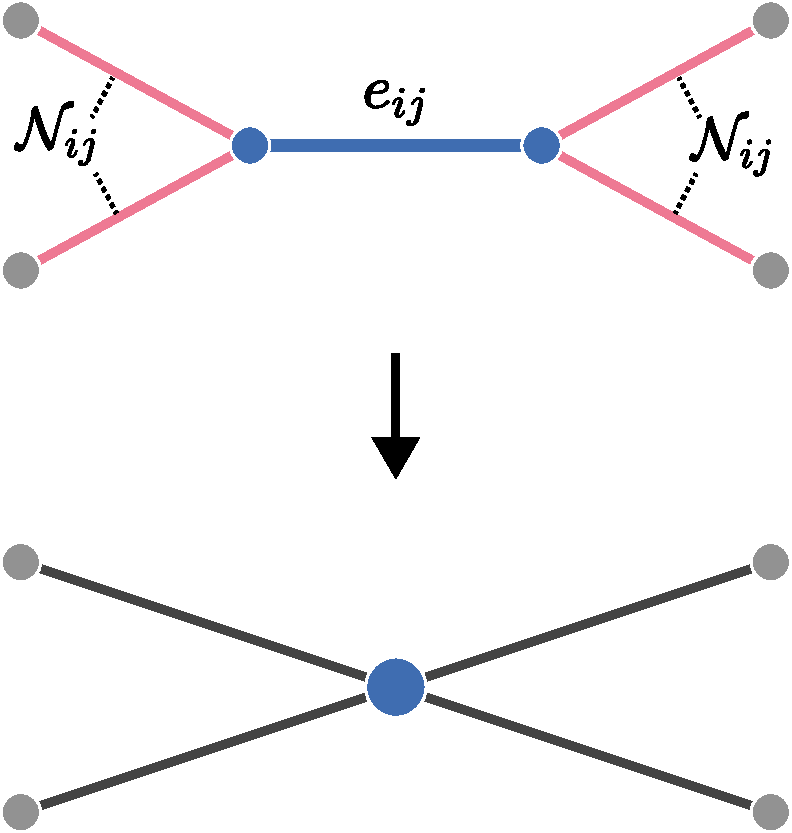
\includegraphics[width=0.75\linewidth]{gfx/coarse/rec.pdf}
			\caption{$\mathit{contract}(G_c, e_{i j})$.}\label{fig:coarse:rec}
		\end{figure}
	\end{minipage}
\end{figure}

We define the neighborhood $\mathcal{N}_{i j}$ as the set of incident edges of $e_{i j}$, including $e_{i j}$ itself;
this is shown as the red and blue edges in \cref{fig:coarse:rec}.
REC only merges vertices that have not been merged with some other vertex yet.
Thus the reduction ratio $r = \frac{N - n}{N}$ is at most $\frac{1}{2}$, i.e.\  $|\mathcal{V}_c| \geq \frac{1}{2} |\mathcal{V}|$.
If the node count needs to be further reduced, REC has to be applied multiple times.
